\documentclass{book}
\title{Microeconomía}
\author{David Gabriel Corzo Mcmath}
\date{2020-Jan-06 11:36:01}
%%%%%%%%%%%%%%%%%%%%%%%%%%%%%%%%%%%%%%%%%%%%%%%%%%%%%%%%%%%%%%%%%%%%%%%%%%%%%%%%%%%%%%%%%%%%%%%%%%%%%%%%%%%%%%%%%%%%%%%%%%%%%%%%%%%%%%%%%%%%%%%
% \usepackage{calc}\usepackage{import}\usepackage{transparent}\usepackage{lipsum}\usepackage{xifthen}\usepackage{xcolor}\usepackage{color}\usepackage{fancyhdr}\usepackage{sectsty}\usepackage{blindtext}\usepackage{xpatch}\usepackage{listing}\usepackage{bookmark}\usepackage{titlesec}\usepackage{spverbatim}\usepackage{lmodern}\usepackage{fancyvrb}\usepackage{fvextra}\usepackage{amssymb}\usepackage{pifont}

\usepackage[margin = 1in]{geometry}
\usepackage{graphicx}
\usepackage{fontenc}
\usepackage{pdfpages}
\usepackage[spanish]{babel}
\usepackage{amsmath}
\usepackage{amssymb}
\usepackage{amsthm}
\usepackage[utf8]{inputenc}
\usepackage{enumitem}
\usepackage{mathtools}
\usepackage{pdfpages}
\usepackage{blindtext}
\usepackage{fancyhdr}
\usepackage{tikz}
\usepackage{hyperref}
\usepackage{longtable}
\usepackage{generalsnips}
\usepackage{calculussnips}
\usepackage{cancel}

\pdfsettings
%%%%%%%%%%%%%%%%%%%%%%%%%%%%%%%%%%%%%%%%%%%%%%%%%%%%%%%%%%%%%%%%%%%%%%%%%%%%%%%%%%%%%%%%%%%%%%%%%%%%%%%%%%%%%%%%%%%%%%%%%%%%%%%%%%%%%%%%%%%%%%%
\begin{document}
\maketitle
\tableofcontents

\chapter{Elasticidad}
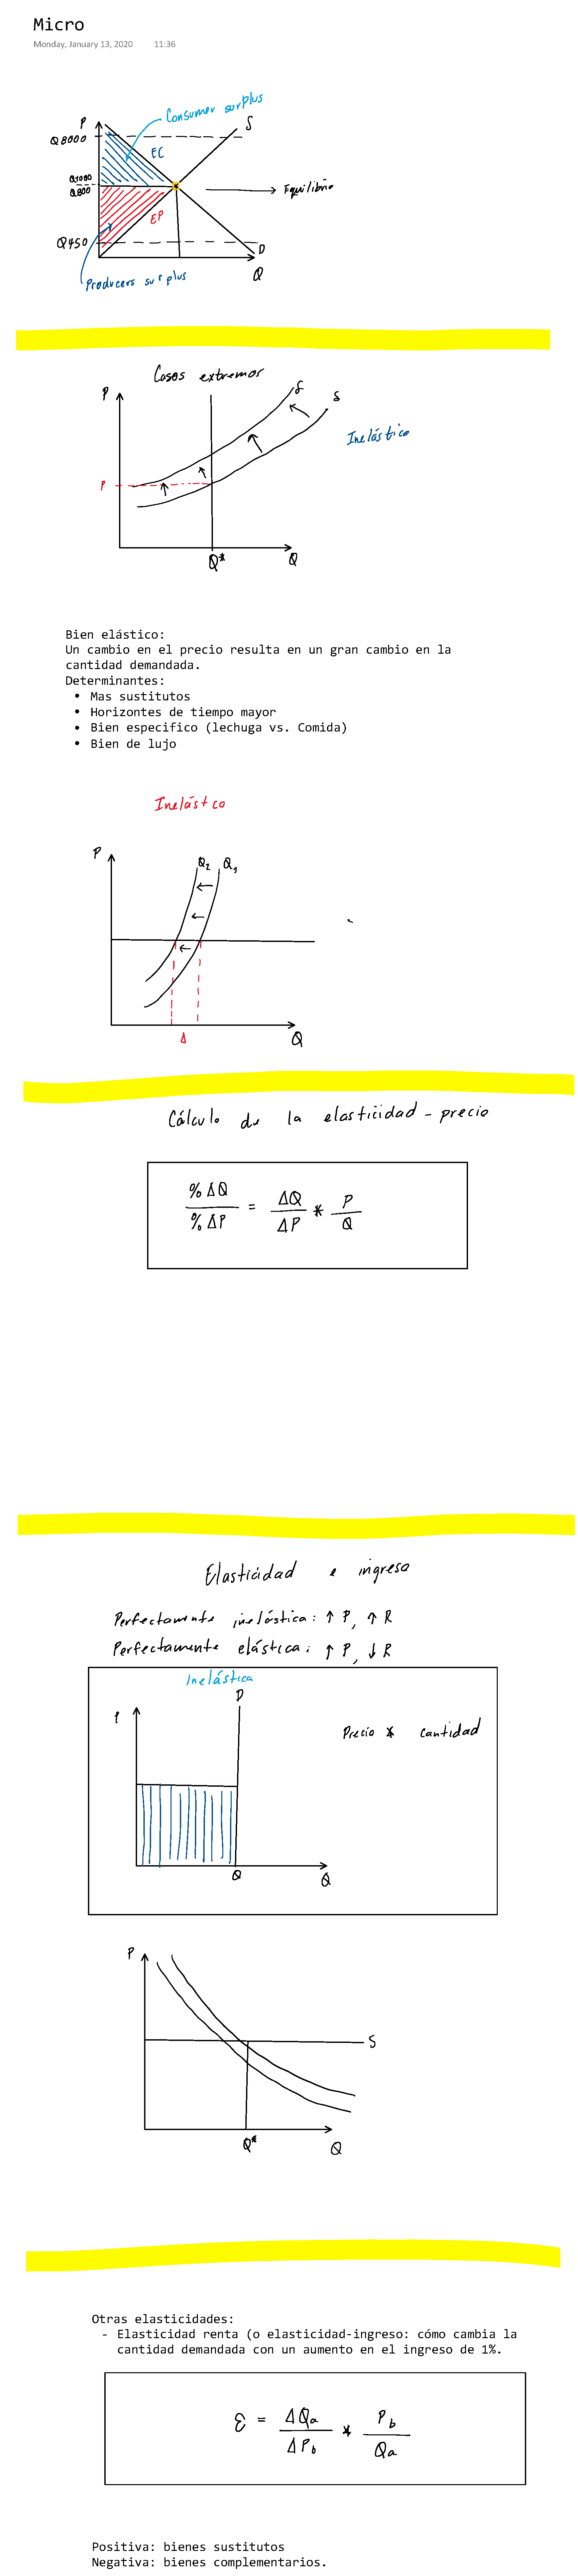
\includepdf[pages=-,pagecommand={\thispagestyle{plain}}]{./Clases/Elasticidad.pdf}
\section{Resolución de corto}
\begin{enumerate}
    
    \item Los tres factores de producción:
        \begin{itemize}
            \item Tecnología de producción. 
            \item Restricciones de costos.
            \item Elecciones de los factores.
        \end{itemize}
    
    \item $Q = 94-2ps+0.2pt+0.4Y$
        \begin{align*}
            \begin{matrix}
                ps=8 \\ 
                pt=10 \\ 
                Y=50 \\ 
            \end{matrix}
        \end{align*}
        \begin{itemize}
            \item Recordar la fórmula de Elasticidad de precio
        \end{itemize}
        \[
            E_P = \frac{\Delta Q}{\Delta P} \times \frac{P}{Q} 
        \]
        \begin{align*}
            \frac{D_{ps}}{D_Q} = -2 \\ 
            E_p = -2 \times \frac{8}{100}  \\ 
            E_p = -0.16 \\ 
        \end{align*}
        \begin{itemize}
            \item $\therefore $ Es una demanda inelástica.
        \end{itemize}
    
    \item $Q=003Y-2p$
        \begin{align*}
            \begin{matrix}
                Y=500 \\ 
                P=\text{  \$  } 5 \\ 
            \end{matrix}
        \end{align*}
        \begin{itemize}
            \item Encontrar la cantidad:
                \begin{align*}
                    q_1 = 0.03(500)-2(5) \\ 
                    q_1 = 5 \\ 
                    \\ 
                    5 = 0.03Y - 2(7) \\ 
                    19 = 0.03Y \\ 
                    \Delta Y = Q_1 \times \Delta p = 5 \times  (7-5) = 10 \\ 
                    \text{  Calcular el nuevo ingreso  } \\ 
                    Y_2 = Y_1 + \Delta Y \\ 
                    Y_2 = 510 \\ 
                    \text{  Calcular la cantidad dos  } \\ 
                    q_2 = 0.03(\underbrace{510}_{Y_2})-s(\underbrace{7}_{p_2}) = -1.3 \\
                    \text{  Efecto sustitución:  } \\ 
                    E_s = q(p_2,y_2)-q(p_1,y_1) \\  
                    E_s = 1.3-5 = -3.7 \\ 
                    \text{  Efecto ingreso:  } \\ 
                    E_i = q(p_2,y_1) - q(p_2,y_2) = 1 -1.3= -0.3 \\ 
                \end{align*}
        \end{itemize}
\end{enumerate}



%%%%%%%%%%%%%%%%%%%%%%%%%%%%%%%%%%%%%%%%%%%%%%%%%%%%%%%%%%%%%%%%%%%%%%%%%%%%%%%%%%%%%%%%%%%%%%%%
\section{Teoría de la empresa}
\begin{itemize}
    \item \textbf{Nos preguntamos:} ¿Es mejor más productividad?
        \begin{itemize}
            \item No siempre, a veces exceden la demanda.
        \end{itemize}    
\end{itemize}


%%%%%%%%%%%%%%%%%%%%%%%%%%%%%%%%%%%%%%%%%%%%%%%%%%%%%%%%%%%%%%%%%%%%%%%%%%%%%%%%%%%%%%%%%%%%%%%%
\section{Las decisiones de producción de empresas}
\begin{itemize}
    \item Las decisiones de producción de una empresa:
    \begin{itemize}
        \item El punto de la teoría del consumidor era maximizar lo que quiere el consumidor.
    \end{itemize}

\end{itemize}


\chapter{Control de precios}
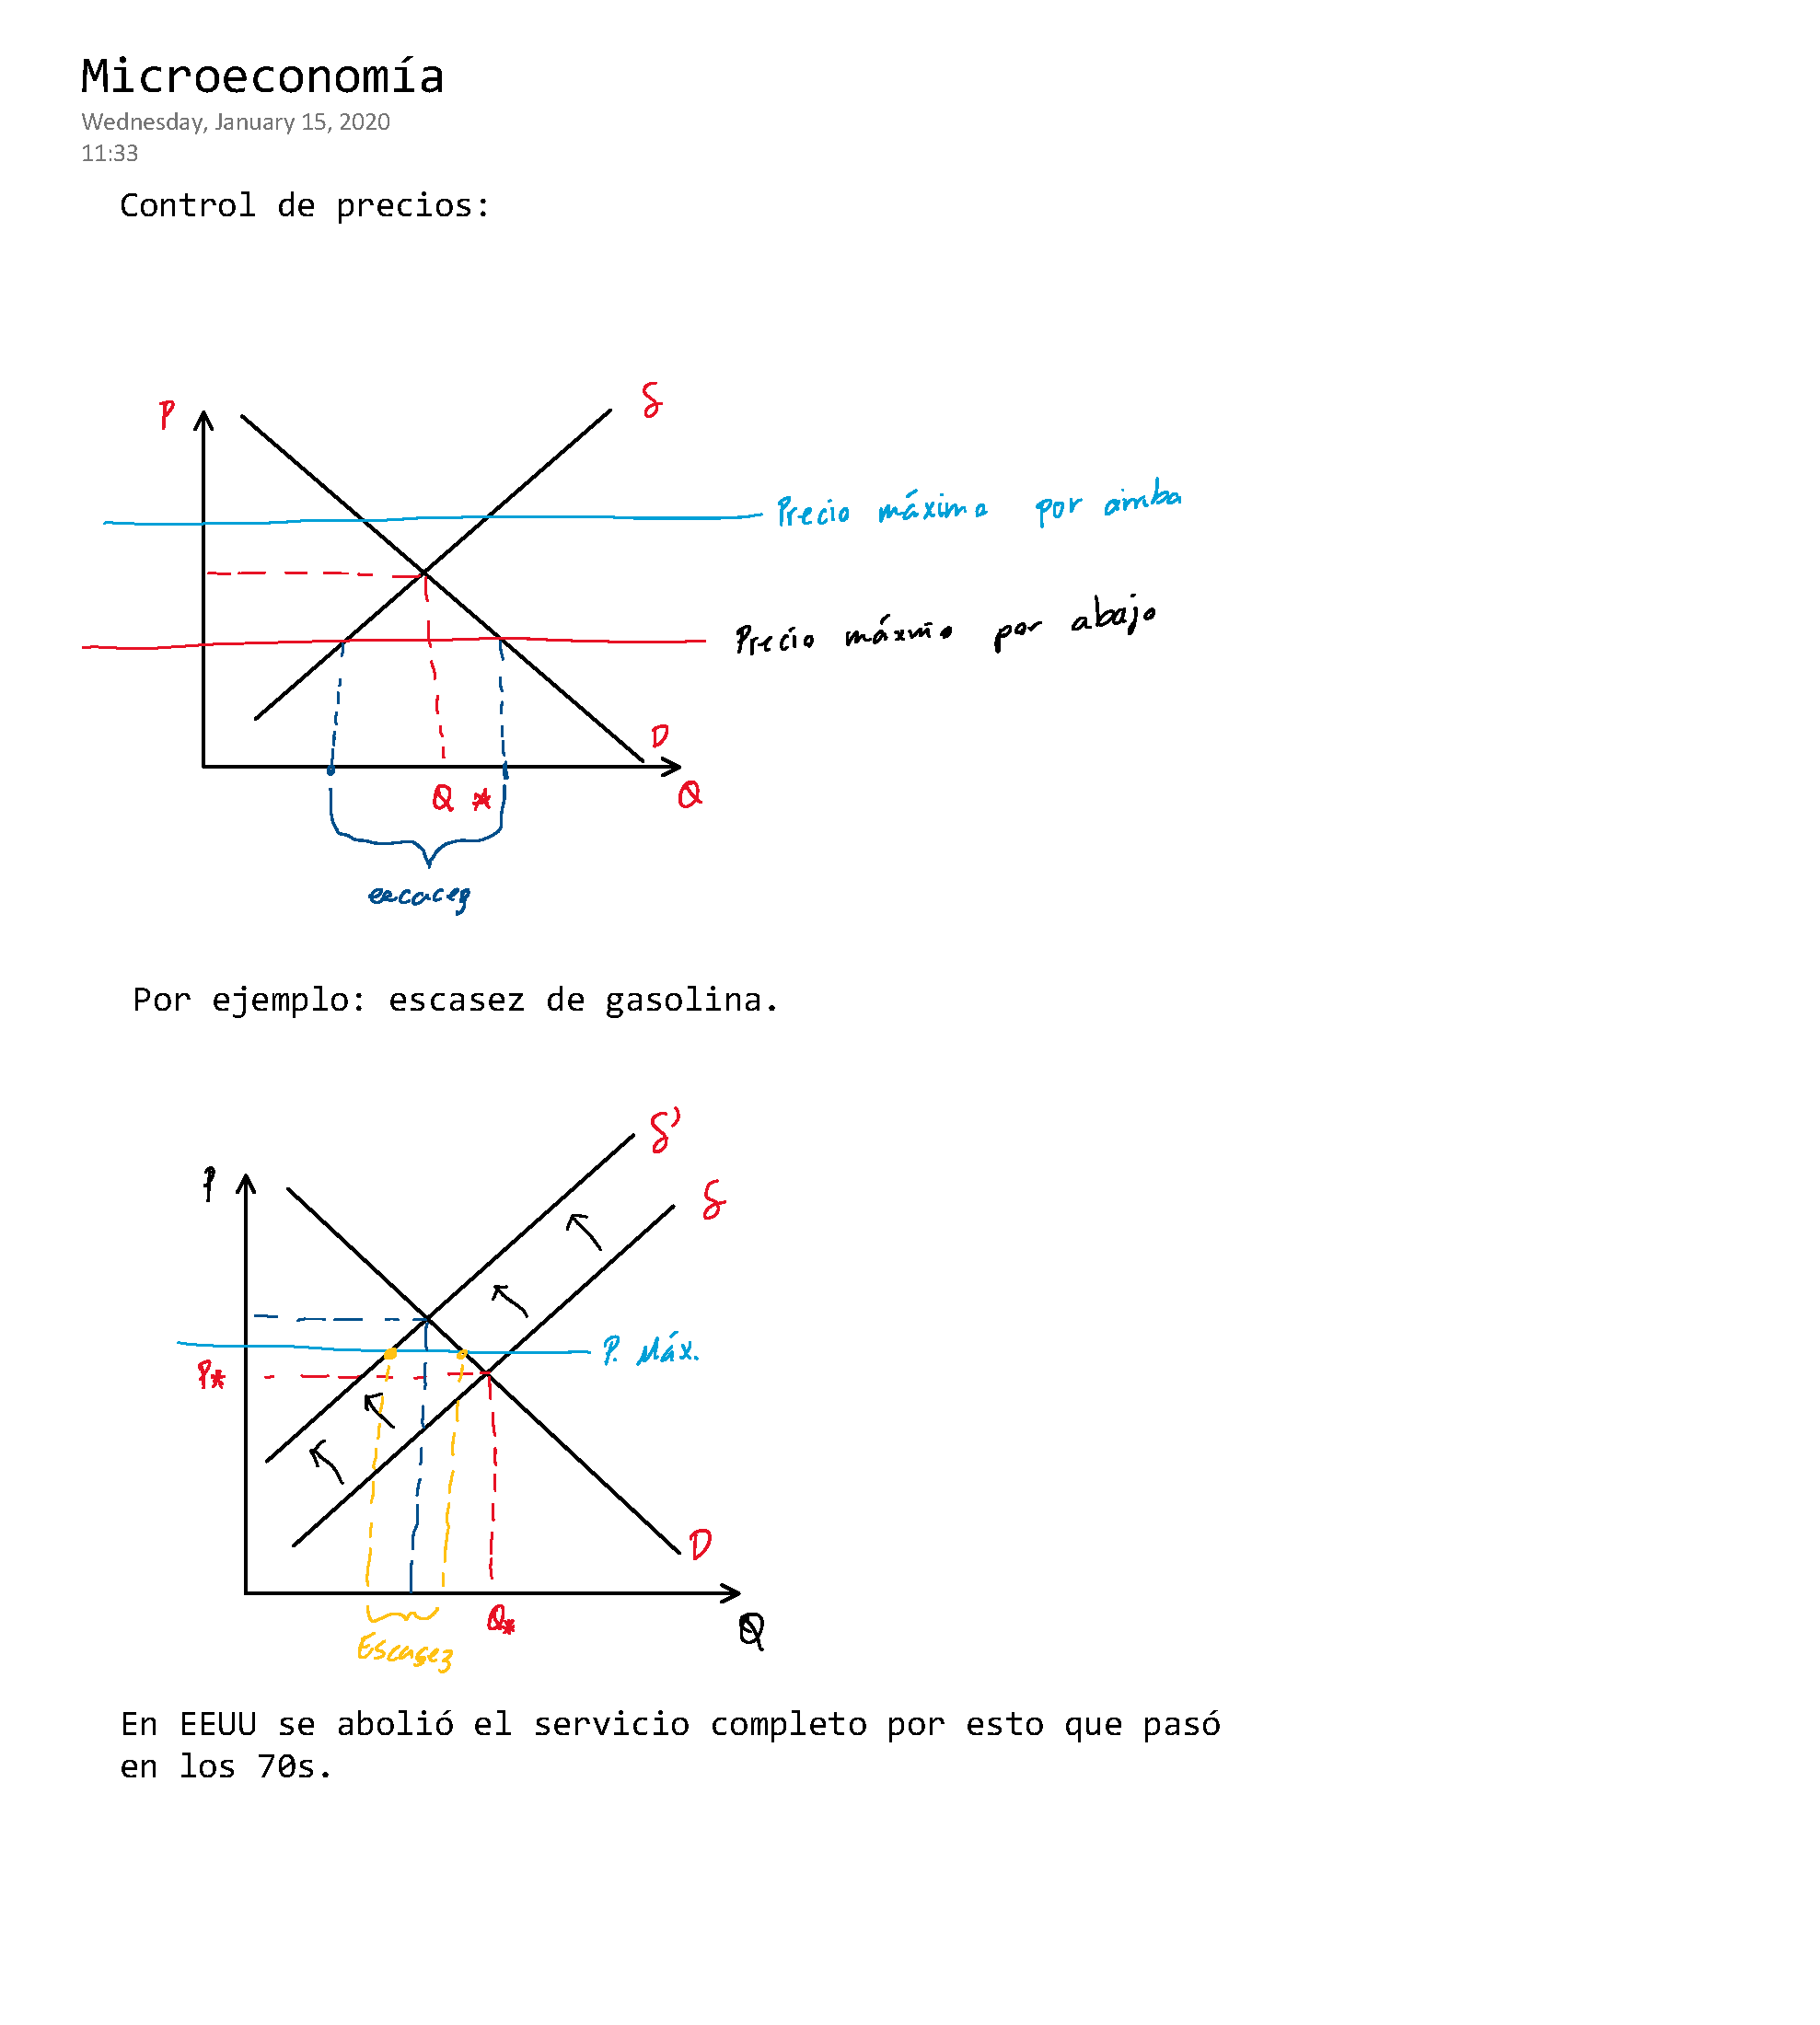
\includepdf[pages=-,pagecommand={\thispagestyle{plain}}]{./Clases/Control_De_PreciosYElasticidad.pdf}
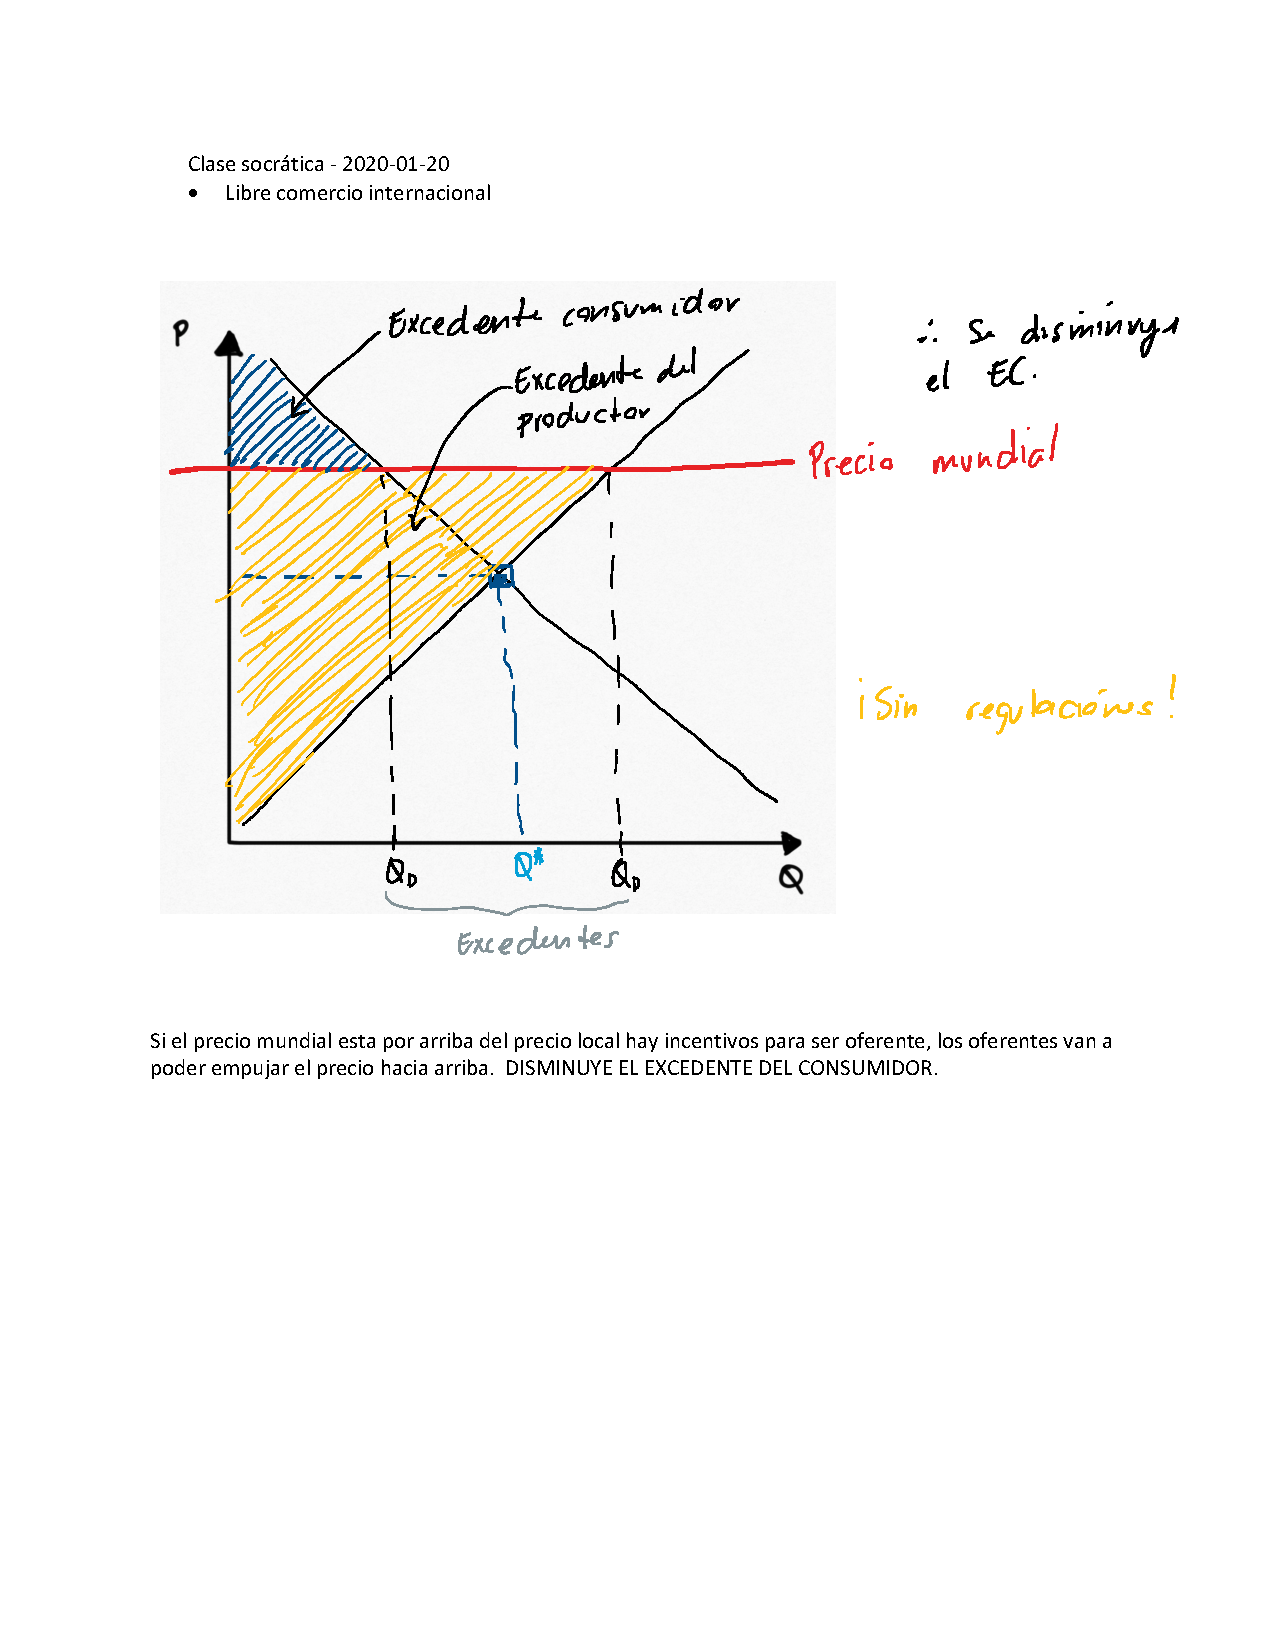
\includepdf[pages=-,pagecommand={\thispagestyle{plain}}]{./Clases/Comercio_Internacional.pdf}
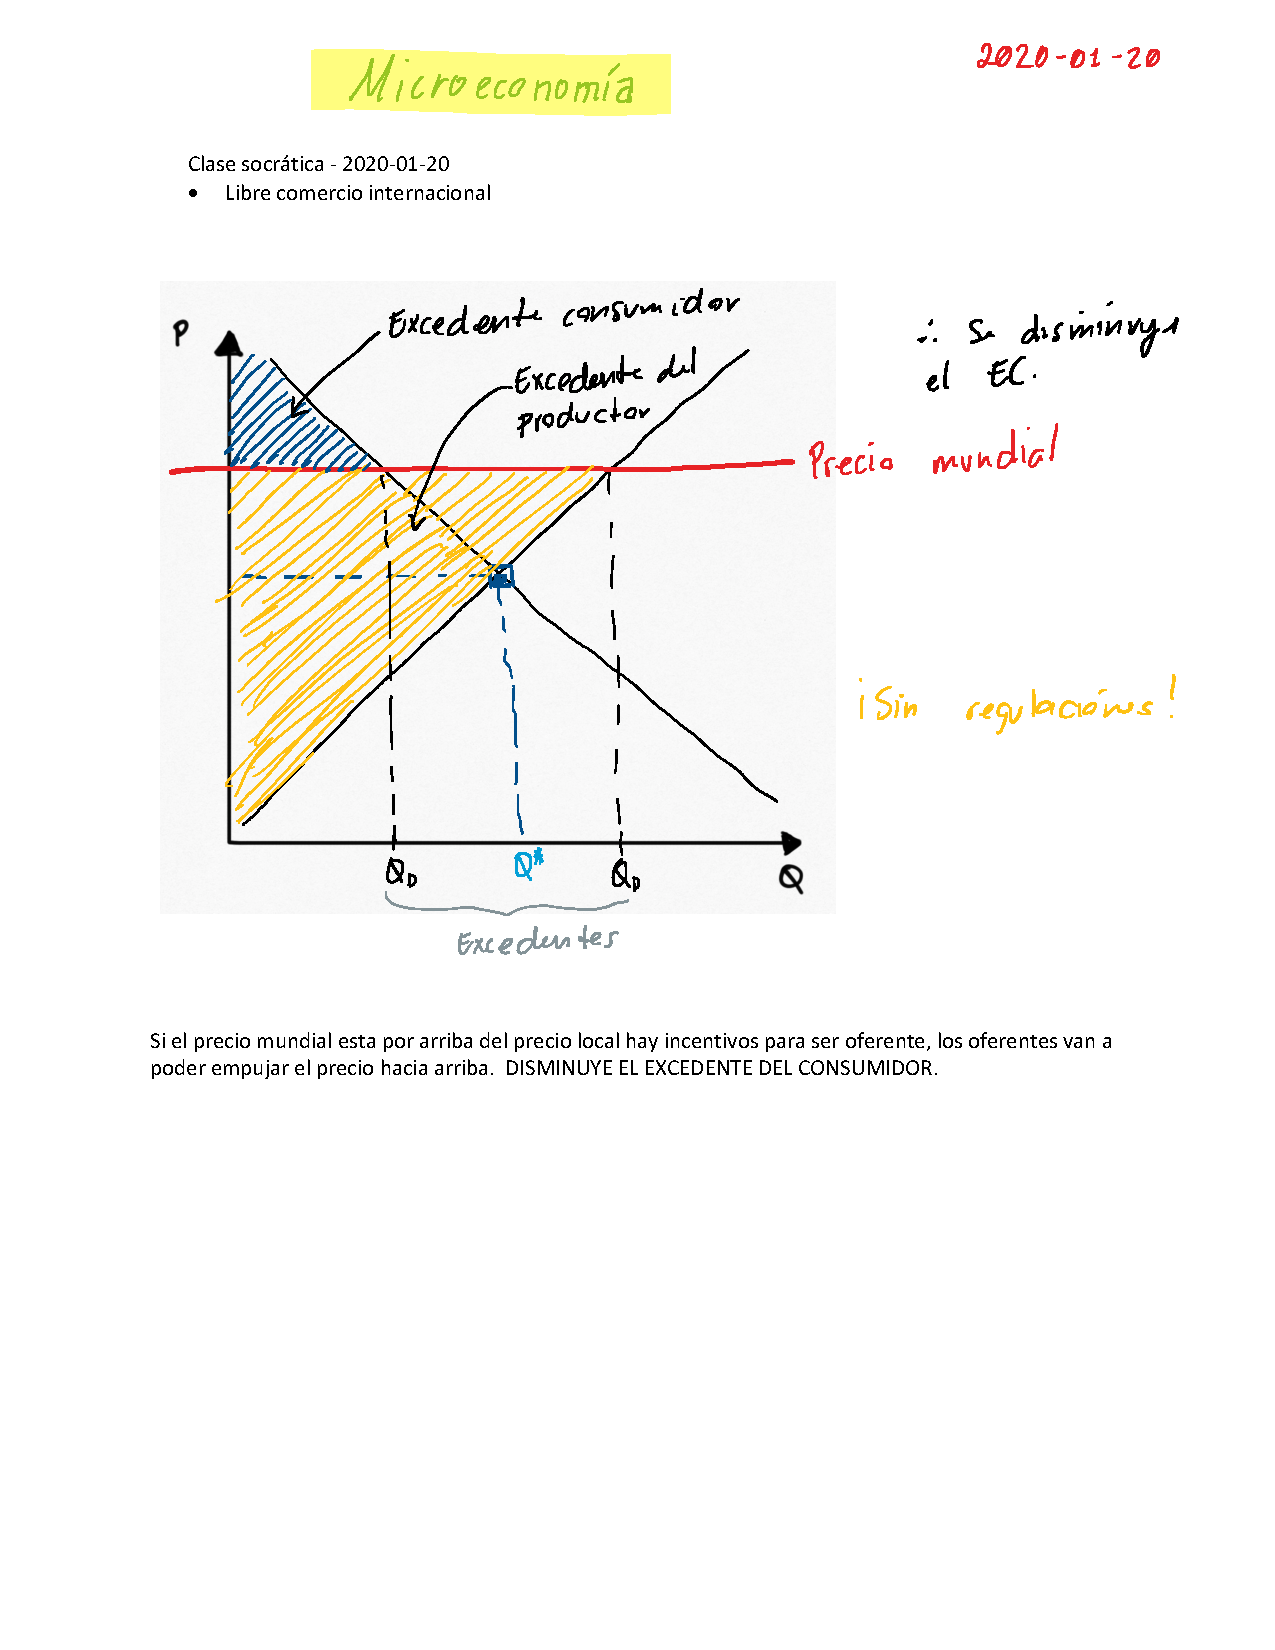
\includepdf[pages=-,pagecommand={\thispagestyle{plain}}]{./Clases/ExcedenteProductoryConsumidor.pdf}

\chapter{Teoría de la empresa y del productor}
% --------------------------------------------------------------------------------------------

\subsection{Los tres factores de producción}
\begin{itemize}
    \item Capital 
    \item Trabajo
    \item Materia Prima 
\end{itemize}

% --------------------------------------------------------------------------------------------

\subsection{Función de producción}
\begin{itemize}
    \item Función de producción: Muestra el nivel de producción máximo que puede obtener la empresa con cada combinación especificada de factores. 
    \item 
\end{itemize}

% --------------------------------------------------------------------------------------------

\subsection{Tiempo}
\begin{itemize}
    \item Corto plazo: asumimos que por lo menos hay un factor que no se pueden alterar, permanece fijo.
    \item Largo plazo: asumimos que todos los factores son variables.
\end{itemize}


%----------------------------------------------------------------------------------------

\subsection{Producción en el corto plazo}
\begin{itemize}
    \item Nivel de producción por unidad de trabajo:
        \[
          \frac{\overbrace{q}^{\text{  Cantidad  }}}{\underbrace{L}_{\text{  Trabajo  }}} 
        \]
    
    \item Producto marginal:
        \begin{itemize}
            \item Marginalmente cuánta productividad deriva aumentar una unidad más de trabajo.
            \item Producto marginal es decreciente.
            \item Hay un punto donde la productividad es óptimo.
        \end{itemize}
        \begin{itemize}[label=\#]
            \item La función de producción en la ida real 
        \end{itemize}
    
    \item Producto medio:
        \begin{itemize}
            \item Siempre que el producto medio esté en aumento el producto marginal estará en aumento, cuando empieza a bajar el producto medio empieza también a bajar el producto marginal.
        \end{itemize}
    
\end{itemize}


%----------------------------------------------------------------------------------------
\subsection{ley de rendimientos marginales decrecientes}
\begin{itemize}
    \item \emph{\textbf{Interesante:} Puede que una empresa esté produciendo más y a pesar en el mismo punto empezar a tener rendimientos marginales decrecientes.}
    \item En el corto plazo los rendimientos productivos son variables: $(K,L)$ , 
\end{itemize}


%----------------------------------------------------------------------------------------
\subsection{Isocuantas}
\begin{itemize}
    \item Es el equivalente a las curvas de indiferencia, estas ilustran indiferencia que tengo al combinar el capital y trabajo y me producen en este caso el mismo output.
    \item La pendiente indica la disposición a intercambiar un factor de producción por otro (TMST).
    \item La isocuanta nos dice que disposición tenemos a sustituir, recordar a la tasa marginal de sustitución, el equvalente en isocuanta es la TMST (Tasa Marginal de Sustitución Técnica).
    \item Recordar el cálculo de la TMS:
        \[
          TMS = -\frac{UM_x}{UM_y} 
        \]
    
    \item El cálculo de TMST:
        \[
          TMST = -\frac{\overbrace{PML}^{\text{  Eje x  }}}{\underbrace{PMK}_{\text{  Eje y  }}} =  
          -\frac{\frac{\Delta q}{\Delta L}}{\frac{\Delta q}{\Delta k} } 
          = -\frac{\Delta q \Delta K }{\Delta q \Delta L} 
          = -\frac{\Delta K}{\Delta L} 
        \]
        \begin{itemize}[label=\#]
            \item L = Trabajo 
            \item K = Capital 
        \end{itemize}
    
    \item Rendimiento de escala, maneras de aumentar la producción:
        \begin{enumerate}
            \item Aumentar en factor y mantener el otro constante ( movimiento de la curva ) 
            \item Disminuir uno de los factores 
            \item Aumentar los dos factores
        \end{enumerate}
    
    \item Cuando se aplican las maneras de aumentar la producción:
        \begin{itemize}
            \item Rendimientos constantes de escala: si duplica los factores se duplica la productividad. 
            \item Rendimientos crecientes de escala: si duplica los factores aumenta más del doble en la productividad.
            \item Rendimientos decrecientes de escala: si duplica los factores ni siquiera llega a la mitad de productividad de más.
        \end{itemize}
\end{itemize}


%----------------------------------------------------------------------------------------

\input{Clases/TeoríaDelProductor.tex}

\chapter{Repaso}
\section{Elasticidad}
\begin{itemize}
    \item Si importan los signos.
    \item 
\end{itemize}


%----------------------------------------------------------------------------------------
\section{Efecto ingreso y sustitución}
\begin{itemize}
    \item Cambia en ingreso:
        \[
          \Delta Y = q_{p_1} \p{p_2-p_1} 
        \]
    
    \item Fórmula de restricción presupuestaria:
        \[
          Y = Q_1P_1+Q_2P_2
        \]
    
    \item Fórmula de nuevo ingreso:
        \[
          Y_2 = Y_1 + \Delta Y
        \]
    
    \item Efecto sustitución: 
        \begin{itemize}
            \item Efecto sustitución es sobre la misma curva.
            \item Se hace una recta paralela a la nueva recta, usar esta para graficar una curva de indiferencia que intersecte dos puntos sobre esta recta.
            \item Si el precio en x disminuye se pivotea a la derecha, si el precio sube se pivotea a la izquierda.
            \item Si el precio y disminuye 
        \end{itemize}
        \[
          E_s = q_2(P_2,Y_2) - q_1(P_2,Y_1)
        \]
    
    \item Efecto ingreso: tengo más poder adquisitivo para comprar.
        \begin{itemize}
            \item El efecto sustitución debe de ser mayor al efecto ingreso, para ser bien inferior.
            \item Bien es inferiores cuando los efectos sustitución y efecto ingreso se mueven en direcciónes opuestas.
            \item Es un bien normal si se mueven en la misma dirección y el punto C está a la derecha.
        \end{itemize}
        \[
          E_y = q_2(P_2,Y_1)-q_1(P_2,Y_2)
        \]
    
    \item Efecto total, Slutsky: 
        \[
          E_T = E_s + E_y
        \]
    
    \item Graficar:
        \begin{itemize}
            \item Hacer una línea paralela a $q_2$
            \item hacer una curva de indiferencia que intersecte a esa paralela en dos puntos
            \item Evaluar si el es un bien normal, inferior o superior.
            \item Un bien giffen es un bien demasiado inferior.
        \end{itemize}
    
    \item Para comprobar si el efecto sustitución:
        \[
          q(P_2) - q(P_1) = \underbrace{E_s + E_y }_{\text{Slutsky} }
        \]
\end{itemize}


%----------------------------------------------------------------------------------------
\section{Teoría del productor \& teoría de consumidor}
\begin{itemize}
    \item Isocoste = Restricción presupuestaria
    \item Isocuanta = Curvas de indiferencia 
\end{itemize}


%----------------------------------------------------------------------------------------
\section{Rendimientos de escala}
\begin{itemize}
    \item La variación debe de ser proporcional y simultánea.
\end{itemize}

%----------------------------------------------------------------------------------------
\section{Costos}
\begin{itemize}
    \item Minimizamos el costo cuando el costo marginal corta el costo medio total. Ó cuando el $C_M = C_{TMe}$ 
    \item Elementos del costo:
        \begin{itemize}
            \item $q$ la función de cantidad.
            
            \item $C_F$: Costo fijo 
                \begin{itemize}
                    \item Ejemplo: $q(x) = 10x + 5$ el $5$ es el costo fijo
                \end{itemize}
            
            \item $C_T$: Costo total
                \begin{itemize}
                    \item Es una función, la derivada es el costo marginal. 
                \end{itemize}
            
            \item Costo medio fijo 
                \begin{itemize}
                    \item Dividir la función de costo total entre $q$:
                        \[
                          C_{CFMe} = \frac{C_F}{q} 
                        \]
                \end{itemize}
            
            \item Costo medio variable 
                \begin{itemize}
                    \item Dividir el costo variable entre $q$
                        \[
                          C_{VMe} = \frac{C_V }{q} 
                        \]
                \end{itemize}
            
            \item Costo medio total 
                \begin{itemize}
                    \item Dividir el costo total entre $q$:
                        \[
                            C_{TMe} = \frac{C_T}{q} 
                        \]
                \end{itemize}
            
            \item Costo marginal:
                \begin{itemize}
                    \item La derivada de la función de costo total, derivar .
                        \[
                          C_M = \frac{\Delta C_T}{\Delta q} 
                        \]
                \end{itemize}
        \end{itemize}
\end{itemize}


%----------------------------------------------------------------------------------------
\section{Dudas}
\begin{itemize}
    \item Lab\#3 Costo de oportunidad (no está claro, solo memorizar el concepto):
        \[
          \text{ Costo de oportunidad } = \text{ Costo de valoración } - \text{ Costo incurrido }
        \]
        \begin{center}
           \begin{tabular}{ | p{5cm} | p{5cm} | }
               \hline
                    Costo & Valoración subjetiva   \\
                \hline
                    \$125 & \$200 \\ 
                    \$50 & \$100 \\ 
               \hline
           \end{tabular}
        \end{center}
\end{itemize}




\end{document}
